En esta secci\'on resolveremos el problema de lectores escritores con prioridad
lectores.\\
Dicho problema consiste en que existe un recurso al que quieren acceder acceder varios procesos, 
unos quieren escribir en el y otros solo leerlo.\\
Los procesos lectores pueden acceder simultaneamente, los escritores solo pueden
escribir secuencialmente (Figura \ref{fig:escritores}).\\


\begin{figure}[!h]
	\centering
	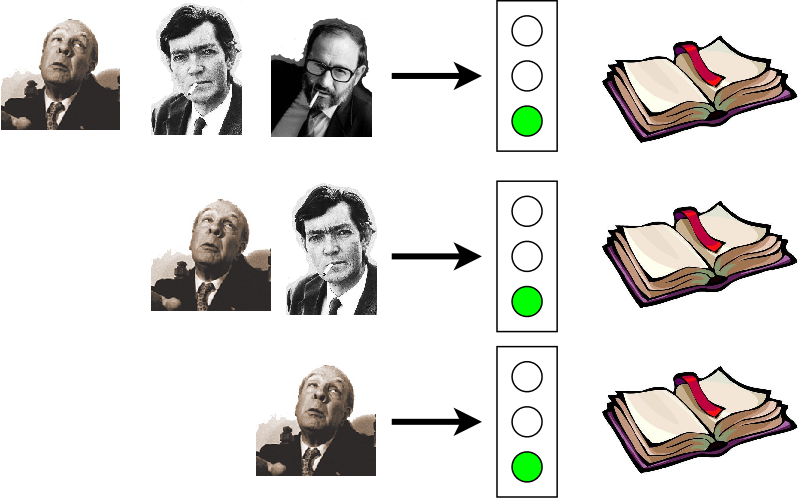
\includegraphics[scale=0.4]{secciones/imagenes/escritores.png}
	\caption{Escritura secuencial}
	\label{fig:escritores}
\end{figure}


Darle prioridad a los lectores por sobre los escritores significa que ning\'un escritor pueda 
escribir mientras haya algun lector queriendo leer (Figura \ref{fig:lectores}).


\begin{figure}[!h]
	\centering
	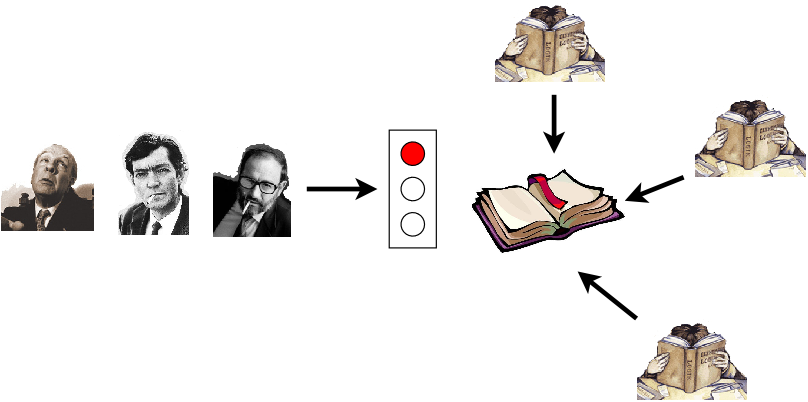
\includegraphics[scale=0.5]{secciones/imagenes/lectores.png}
	\caption{Lectura simult\'anea con bloqueo de escritores}
	\label{fig:lectores}
\end{figure}

\subsection{Arquitectura}
Para implementar nuestra soluci\'on utilizamos dos sem\'aforos, uno para restrigir el acceso
de los escritores ($SemaforoEscritores$) y otro para el \'area de memoria compartida donde guardamos la 
cantidad de lectores ($AccesoCantLectores$).

\subsection{Algoritmo}
Todo comienza con dos ciclos que crean procesos lectores y procesos escritores para que compitan entre s\'i.

\subsubsection{Proceso Lector}
Este es el pseudoc\'odigo del proceso lector, lo que hace es antes de leer aumentar la cantidad de lectores, si es
el primer proceso lector tiene que bloquear el acceso a los escritores, y si es el \'ultimo tiene que desbloquearlo.

\begin{scriptsize} 
\begin{verbatimtab} 
	
    LoopForEver
        P(AccesoCantLectores)
            lectores++

                /* Si es el primer lector tiene que bloquear a los escritores  */
            
                Si(lectores == 1)
                   P(SemaforoEscritores)
                Fin Si
        
        V(AccesoCantLectores)

        Leer
        
        P(AccesoCantLectores)
            lectores--
                
                /* Si es el ultimo lector tiene que desbloquear a los escritores  */
                
                Si(lectores == 0)
                   V(SemaforoEscritores)
                Fin Si

        V(AccesoCantLectores)
    End Loop

\end{verbatimtab}
\end{scriptsize}


\subsubsection{Proceso Escritor}
El proceso escritor solamente trata de escribir, para eso usa el sem\'aforo $SemaforoEscritores$.


\begin{scriptsize} 
\begin{verbatimtab} 
	
    LoopForEver
        P(SemaforoEscritores)
            Escribir
        V(SemaforoEscritores)
    End Loop

\end{verbatimtab}
\end{scriptsize}

\subsection{Localizaci\'on del c\'odigo y ejemplos}

En el directorio \emph{/usr/tp/13} se encuentran los fuentes del ejercicio y un ejecutable llamado \emph{compex} 
que muestra como compilar indicando las diferentes cantidades de lectores y escritores.\\

\subsubsection{Ejemplo 1 - Solo Escritores}

En el siguiente ejemplo mostramos que el algorítmo permite solamente operar a un escritor a la vez. 
Se han suprimido los lectores y se han utilizado cuatro escritores.\\
El ejecutable se llama \emph{soloEscritores}.


\begin{scriptsize} 
\begin{verbatimtab} 


[E 2] Permiso escribir?
[E 1] Permiso escribir?
[E 0] Permiso escribir?
[E 3] Escritura finaIizada
[E 2] Permiso escribir otorgado
[E 2] Escritura finaIizada
[E 1] Permiso escribir otorgado
[E 1] Escritura finaIizada
[E 0] Permiso escribir otorgado
[E 3] Permiso escribir?
[E 2] Permiso escribir?
[E 1] Permiso escribir?
[E 0] Escritura finaIizada
[E 3] Permiso escribir otorgado
[E 0] Permiso escribir?
[E 3] Escritura finaIizada
[E 2] Permiso escribir otorgado
[E 2] Escritura finaIizada
.....
\end{verbatimtab}
\end{scriptsize} 

\subsubsection{Ejemplo 2 - Solo Lectores}
Ahora mostramos que los lectores pueden leer todos al mismo tiempo, utilizamos cinco lectores y ningun escritor.\\
El archivo de pruebas se llama \emph{soloLectores}


\begin{scriptsize} 
\begin{verbatimtab}

[L 4] Queriendo leer
Aumentando Lectores, ahora hay 1
A partir de ahora Bloqueamos Escritores
---------------------------------------
[L 4] Comenzado Lectura
[L 3] Queriendo leer
Aumentando Lectores, ahora hay 2
[L 3] Comenzado Lectura
[L 2] Queriendo leer
Aumentando Lectores, ahora hay 3
[L 2] Comenzado Lectura
[L 1] Queriendo leer
Aumentando Lectores, ahora hay 4
[L 1] Comenzado Lectura
[L 0] Queriendo leer
Aumentando Lectores, ahora hay 5
[L 0] Comenzando Lectura
[L 4] Finalizando Lectura
Disminuyendo Lectores, ahora hay 4
[L 3] Finalizando Lectura
Disminuyendo Lectores, ahora hay 3
[L 2] Finalizando Lectura
Disminuyendo Lectores, ahora hay 2
[L 1] Finalizando Lectura
Disminuyendo Lectores, ahora hay 1
[L 0] Finalizando Lectura
Disminuyendo Lectores, ahora hay 0
.....
\end{verbatimtab}
\end{scriptsize}

\subsubsection{Ejemplo 3 - Lectores Vs. Escritores}
Para finalizar utilizamos a cinco lectores y tres escritores, se quitaron los mensajes de los sem\'aforos para 
comodidad en la lectura y se intercalaron comentarios en el seguimiento.

\begin{scriptsize}
\begin{verbatimtab}

[L 4] Queriendo leer
Aumentando Lectores, ahora hay 1
A partir de ahora Bloqueamos Escritores
---------------------------------------
[L 4] Comenzado Lectura
[L 3] Queriendo leer
Aumentando Lectores, ahora hay 2
[L 3] Comenzado Lectura
[L 2] Queriendo leer
Aumentando Lectores, ahora hay 3
[L 2] Comenzado Lectura
[L 1] Queriendo leer
Aumentando Lectores, ahora hay 4
[L 1] Comenzado Lectura
[L 0] Queriendo leer
Aumentando Lectores, ahora hay 5
[L 0] Comenzando Lectura

--Como hay lectores los escritores quedan encolados

[E 2] Permiso escribir?
[E 1] Permiso escribir?
[E 0] Permiso escribir?

[L 4] Finalizando Lectura
Disminuyendo Lectores, ahora hay 4
[L 3] Finalizando Lectura
Disminuyendo Lectores, ahora hay 3
[L 2] Finalizando Lectura
Disminuyendo Lectores, ahora hay 2
[L 1] Finalizando Lectura
Disminuyendo Lectores, ahora hay 1
[L 0] Finalizando Lectura
Disminuyendo Lectores, ahora hay 0
Ultimo lector, ahora entran escritores
--------------------------------------
[E 2] Permiso escribir otorgado
[L 0] Queriendo leer
Aumentando Lectores, ahora hay 1
A partir de ahora Bloqueamos Escritores
---------------------------------------

-- Los escritores 2, 1 y 0 quedaron encolados antes de la entrada del nuevo lector, por lo que primero
-- deben terminar antes de que los lectores puedan leer

[E 2] Escritura finalizada
[E 1] Permiso escribir otorgado
[E 1] Escritura finalizada
[E 0] Permiso escribir otorgado

-- Los escritores 2 y 1 quieren volver a escribir y no van a poder porque ya se habia bloqueado la entrada,
-- por lo que quedan encolados y comienzan los lectores

[E 2] Permiso Escribir?
[E 1] Permiso Escribir?
[E 0] Escritura finalizada
[L 0] Comenzando Lectura
[L 1] Queriendo leer
Aumentando Lectores, ahora hay 2
[L 1] Comenzando Lectura
[L 2] Queriendo leer
Aumentando Lectores, ahora hay 3
[L 2] Comenzando Lectura
[L 3] Queriendo leer
Aumentando Lectores, ahora hay 4
[L 3] Comenzando Lectura
[L 4] Queriendo leer
Aumentando Lectores, ahora hay 5
[L 4] Comenzando Lectura
[L 3] Finalizando Lectura
Disminuyendo Lectores, ahora hay 4
[L 2] Finalizando Lectura
Disminuyendo Lectores, ahora hay 3
[L 1] Finalizando Lectura
Disminuyendo Lectores, ahora hay 2
[L 0] Finalizando Lectura
Disminuyendo Lectores, ahora hay 1
[E 0] Permiso Escribir?
[L 4] Finalizando Lectura
Disminuyendo Lectores, ahora hay 0
Ultimo lector, ahora entran escritores
--------------------------------------
[E 2] Permiso escribir otorgado 
[L 0] Queriendo leer
Aumentando Lectores, ahora hay 1
A partir de ahora Bloqueamos Escritores
---------------------------------------
[E 1] Permiso escribir otorgado
[E 1] Escritura finalizada
[E 0] Permiso escribir otorgado
[E 2] Permiso Escribir?
[E 0] Escritura finalizada
[L 0] Comenzando Lectura
.....

\end{verbatimtab}
\end{scriptsize}
